\documentclass[a4paper,12pt]{jsarticle}

% 数式
\usepackage{amsmath,amsfonts}
\usepackage{bm}
% 画像
\usepackage[dvipdfmx]{graphicx}

\usepackage{listingsutf8,jlisting} %日本語のコメントアウトをする場合jlistingが必要
%ここからソースコードの表示に関する設定
\lstset{
  basicstyle={\ttfamily},
  identifierstyle={\small},
  commentstyle={\smallitshape},
  keywordstyle={\small\bfseries},
  ndkeywordstyle={\small},
  stringstyle={\small\ttfamily},
  frame={tb},
  breaklines=true,
  columns=[l]{fullflexible},
  numbers=left,
  xrightmargin=0zw,
  xleftmargin=3zw,
  numberstyle={\scriptsize},
  stepnumber=1,
  numbersep=1zw,
  lineskip=-0.5ex
}

\begin{document}

\title{コンパイラ 演習課題}
\author{坪井正太郎(101830245)}
\date{\today}
\maketitle
\subsection*{1}
\[\left\{V_0, V_2, V_5\right\}\]

\subsection*{2}
Gが木ならば,1つを除いて各頂点はただ1つの先行頂点を持つ。
先行頂点の数は有効辺の個数に等しいので,Vの要素数がnならば,Eの要素数はn-1になる。

\subsection*{3}
\subsubsection*{(1)}
\begin{figure}[htb]
  \begin{center}
  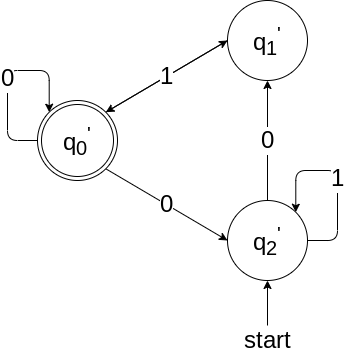
\includegraphics[width=5cm]{1.png}
  \end{center}
\end{figure}

\subsubsection*{(2)}
Lを正規表現で表すと,\[(0|1)^* 0^* 1 (11)^* 0 1^*\]となる。
これが,$ww^R$のように対照な文になっているので,どこを対照の中心に取るか分けて考える。
($ww^R\in L$)

$1^*→1^*,01^*→1^*001^*$となり,Lの表現を満たさない。
次に$1 (11)^*$の部分のどこが$ww^R$の中心になるとしても,1が偶数個だけ続き,Lの表現を満たさない。
また,これより前の部分で中心になっている場合,明らかに$w^R$の部分のみでLを満たしている。

つまり,\[ww^R\in L \rightarrow w^R\in L\]

よって,$M^R$で識別できる。
(図は(1)と同じなので略)\\
※一般のLに対しては明らかに成り立たない。その場合,$M^R$がわかっているならば,$M$と同時に操作して,その時の各状態である,$(q_i, {q_j}^{dash})$を状態にもつオートマトンを考え,i=jで受理させる。

\newpage

\subsection*{4}
各桁の和をmod3で分けて考える。
\subsubsection*{(a)}
\begin{figure}[htb]
  \begin{center}
  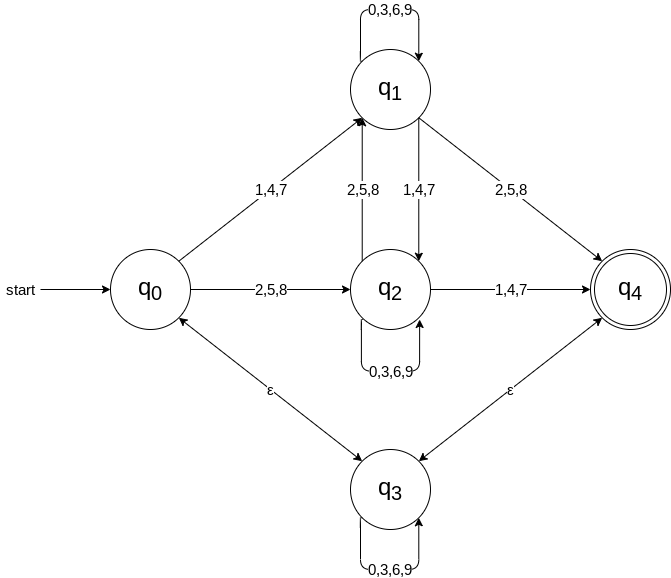
\includegraphics[width=\linewidth]{4-a.png}
  \end{center}
\end{figure}

\newpage
\subsubsection*{(b)}
\begin{figure}[htb]
  \begin{center}
  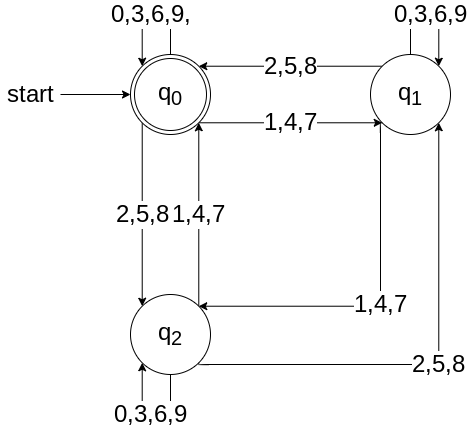
\includegraphics[width=8cm]{4-b.png}
  \end{center}
\end{figure}



\end{document}
